\begin{figure*}[!h]
  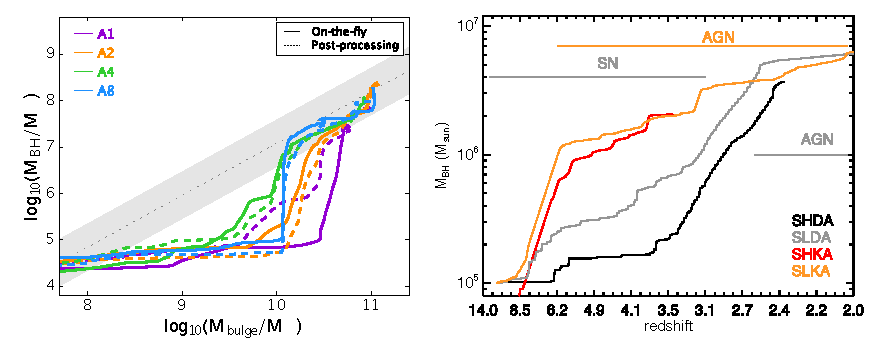
\includegraphics[width=\textwidth]{figures/comparisonfig.pdf}
    \caption{Black hole growth figures reproduced from A17 (left) and D15 (right).
    Unfortunately the data was not available scaled with the same property
    (note that on the left black hole mass is plotted with bulge mass, and on
    the right with redshift), but assuming that the bulge grows in a regular
    way with redshift both of these plots show a very similar black hole growth
    history.}
  \label{fig:bhhistory}
\end{figure*}
As mentioned in §\ref{sec:models}, there is no treatment of black holes or AGN
in the original \fire{} project. After the main runs, though, A17 looked at the
effects of star formation on the growth of the black hole; this still did
not include any treatment of AGN feedback. The \hagn{} project, on the other
hand, was based almost entirely around the effects of AGN on galaxies and
vice-versa, and hence it is expected that their treatment is more precise.
D15 in particular looks at the effects of star formation on black hole growth,
and hence this is directly comparable with A17.

The two projects use remarkably different models for their black hole growth.
D15 implements black hole growth using \citet{bondi_spherically_1952} such
that
\begin{align}
  \dot{M}_{BH} = 4\pi \alpha G^2 M_{BH}^2
                 \frac{\bar{\rho}}{(c_s^2 + u^2)^{3/2}},
  \label{eqn:d15:mdot}
\end{align}
where $\alpha$ is a boost factor constant, $G$ the gravitational constant,
$\bar{\rho}$ is the local mean density of gas around the black hole, $c_s$ the
local sound speed, and $u$ the average gas velocity relative to the black hole.
A17 uses the `torque' model from \citet{hopkins_analytic_2011} such that
\begin{align}
  \dot{M}_{BH} = (1 - \eta) \epsilon f_d^{5/2} M_d R_0^{-3/2} M_{BH}^{1/6}~,
  \label{eqn:a17:mdot}
\end{align}
where $f_d$ and $M_d$ are the mass fraction and total mass of the disks within
a radius of $R_0$ which encloses 256 gas particles.
Note that, due to the bulge mass-black hole mass relation,
\citep{haring_black_2004} essentially scales like
$\dot{M_{BH}} \propto M_{BH}^{4/3}$.

In Figure \ref{fig:bhhistory} the accretion histories of the two black holes
in both papers is shown. It is remarkable that despite very different
`feeding' models, they arrive at a very similar accretion history; this is due
to the fact that in both models, the accretion is limited by the effects
of star formation.

